%%
%% This is file `mcmthesis-demo.tex',
%% generated with the docstrip utility.
%%
%% The original source files were:
%%
%% mcmthesis.dtx  (with options: `demo')
%% 
%% -----------------------------------
%% 
%% This is a generated file.
%% 
%% Copyright (C)
%%       2010 -- 2015 by Zhaoli Wang
%%       2014 -- 2019 by Liam Huang
%%       2019 -- present by latexstudio.net
%% 
%% This work may be distributed and/or modified under the
%% conditions of the LaTeX Project Public License, either version 1.3
%% of this license or (at your option) any later version.
%% The latest version of this license is in
%%   http://www.latex-project.org/lppl.txt
%% and version 1.3 or later is part of all distributions of LaTeX
%% version 2005/12/01 or later.
%% 
%% This work has the LPPL maintenance status `maintained'.
%% 
%% The Current Maintainer of this work is latexstudio.net.
%% 
%%
%% This is file `mcmthesis-demo.tex',
%% generated with the docstrip utility.
%%
%% The original source files were:
%%
%% mcmthesis.dtx  (with options: `demo')
%%
%% -----------------------------------
%%
%% This is a generated file.
%%
%% Copyright (C)
%%       2010 -- 2015 by Zhaoli Wang
%%       2014 -- 2019 by Liam Huang
%%       2019 -- present by latexstudio.net
%%
%% This work may be distributed and/or modified under the
%% conditions of the LaTeX Project Public License, either version 1.3
%% of this license or (at your option) any later version.
%% The latest version of this license is in
%%   http://www.latex-project.org/lppl.txt
%% and version 1.3 or later is part of all distributions of LaTeX
%% version 2005/12/01 or later.
%%
%% This work has the LPPL maintenance status `maintained'.
%%
%% The Current Maintainer of this work is Liam Huang.
%%
\documentclass{mcmthesis}
\mcmsetup{CTeX = false,   % 使用 CTeX 套装时,设置为 true
        tcn =2104419, problem = D,
        sheet = true, titleinsheet = true, keywordsinsheet = true,
        titlepage = false, abstract = true}
\usepackage{newtxtext}%\usepackage{palatino}
\usepackage{lipsum}%用于生成随机文本,实际写作可以去掉
\usepackage{booktabs}
\usepackage{graphicx}  %插入图片的宏包
\usepackage{float}  %设置图片浮动位置的宏包
\usepackage{subfigure}  %插入多图时用子图显示的宏包
\usepackage{setspace}
\newcommand{\upcite}[1]{\textsuperscript{\textsuperscript{ \cite{#1}}}}
\title{\large\textbf{The Infectivity of Music: A Comprehensive Perspective} }
\date{\today}
\begin{document}
\begin{abstract}
	\begin{spacing}{0.8}
Music has the power to strike deep in the heart, which has intoxicated generations for thousands of years. The work of a musician will affect not only the emotions of the audience, but also the creation of other musicians. In this paper, our team are asked to build models to understand and measure the impact of previous music on later musicians and their creations. 

Before modeling, we preprocess the given data to ensure the integrity and validity of it. For missing data, we use cubic spline interpolation to complete it.

In order to visualize the relationship between influencers and followers, we use a variety of elements including circle, arrow, line and so on to draw a global network diagram mainly reflecting the influence of various music genres, and a subnetwork reflecting the influence of musicians on other people or genres. Aim to quantify the influence, we define six parameters from the depth, speed and breadth of influence to quantitatively describe the influence. And show them in the global network and subnetwork through the color and arrow shape, which ensure the intuitiveness and readability of the network diagram.

Further, we establish the similarity comprehensive comparison model to develop measures of the similarity of artists within and between genres. First, the factor analysis method is used to reduce the dimension of variables to extract the feature vectors of each artist; Second, after comprehensively comparing various similarity measures, the modified cosine similarity is selected as the main index to evaluate the similarity of artists, which not only considers the direction relationship of multi-dimensional vector space, but also takes into account the size of the difference. According to the index, the intraclass similarity and inter-class similarity are calculated, which are used to construct the similarity matrix reflecting the degree of similarity. Finally, sort the similarity and draw a conclusion that for most genres, artists within genre are more similar than artists between genres.

Then, we use Duncan method to judge the significant value of 20 genres corresponding to each music feature, and take the mean value as the main index to measure the fluctuation of music features. The speechiness and instrumentalness are selected as the features to distinguish genres. In order to describe the changes of genres over time, a time series diagram is drawn. And to find out the related genres, it is found that there is a close relationship between country music and children’s music through inter-class similarity ranking. For question 4, the similarity matrix is recalculated when only influencers and followers are considered, and the promotion rate is calculated, which shows that influencers really have an impact on followers. Based on the same idea, the similarity matrix of each index is calculated, and the promotion rate is obtained, which indicates danceability is the most ‘contagious’ characteristic.

To find out the artists who represent the music revolutionaries, the jump point is determined by the time series diagram. Before the jump point, the screening range is narrowed according to the characteristics of the genre. The similarity between the influencers and followers in the range is calculated, and the threshold is set to determine the number of effective followers of the influencers. By sorting, it is found that the Beatles and Bob Dylan can be called revolutionaries.
For pop music, the number of effective followers and dynamic correlation are used as evaluation indexes to find out the dynamic influencers in different periods and explain the sequence diagram of characteristics.

Finally, considering the relevant background, we analyze the influence of society, politics and technology on music.
\end{spacing}


\begin{keywords}
network; decomposition; similarity; Duncan method; revolutionary
\end{keywords}
\end{abstract}
\maketitle
\begin{spacing}{0.5}  %更改括号内公式的行距,最前面要加setspace宏包
\tableofcontents
\end{spacing}
\newpage
%% Generate the Table of Contents, if it's needed.
%% \tableofcontents
%% \newpage
%%
%% Generate the Memorandum, if it's needed.
%% \memoto{\LaTeX{}studio}
%% \memofrom{Liam Huang}
%% \memosubject{Happy \TeX{}ing!}
%% \memodate{\today}
%% \logo{\LARGE I'm pretending to be a LOGO!}
%% \begin{memo}[Memorandum]
%%   \lipsum[1-3]
%% \end{memo}
%%
\section{Introduction}
\subsection{Problem background}
 Music is the art of expressing emotion with sound, which can change the emotional tone of the work through differences in rhythm, melody, speed and other elements. As an important bridge to communicate with people from all over the world, music can resolve misunderstandings, strengthen unity, and soothe the soul, which make it an important part of culture. Looking back at the history of world music, different music genres have been leading the way for decades, influencing the music creation of latecomers and also affect each other, which form a colorful music world. 

In that case, aim to explore the development of world music, it's necessary to study the influence of previous music on new music and musicians. With the data provided by the ICM, our team is asked to create a model to measures musical influence in the past decades, while making research on the evolution and revolutionary trends of artists and genres.


\subsection{Overview of our goals}
\begin{itemize}
	\item Create a music influence network to connect influencers and followers, while designing parameters to describe its subnet. And identify the effects of social, political or technological 
	changes within the network.
	\item Develop measures of music similarity to determine whether the artists within genre more similar than the ones between genres.
	\item Expounds the differences and relations between music genres, and studies the development of them.
	\item Find out whether the influencer really affects the creation of followers and explain the reason. 
	\item Identify indicators that can signify musician revolutions and change makers, study the development process of one of the genres.
\end{itemize}
\section{Assumptions}
\noindent%取消单段缩进
\textbf{Assumptions}

\begin{itemize}
	\item The data given in the file are completely true and reliable.
	\item Ignore the influence of musicians' personal factors on creation.
	\item Assumed that all music feature data are properly quantified
\end{itemize}
\section{Data Processing}
By analyzing the data in the table, we find that some data are zero for a period of time, which we regard as missing data. In order to solve this problem, we use cubic spline method for interpolation fitting to fill in the exact data and ensure the data integrity.
\section{Network of Musical Influence}
\subsection{Global Network} 
The global network diagram is a comprehensive reflection of the influence and the relationship between all artists and all genres. In order to express their mutual influence intuitively and clearly, we create three composition elements as follows.
\begin{itemize}
	\item \textbf{Genre circle}. It contains all artists of the same genre. The more artists included, the bigger the genre circle.
	\item \textbf{Individual circle}. It represents an artist, which is distinguished by color in genre circle.
	\item \textbf{Line}. The line indicates the influence of one genre to another and  the color of which represents the genre it comes from. The thickness of the line represents the number of people in a genre that is affected by another genre. In other words, the thicker the line, the greater the degree of influence.
	\item \textbf{Arrow}. The arrow shows the artist’s influence on other artists.
\end{itemize}
\begin{figure}[H]%图片
	\small
	\centering
	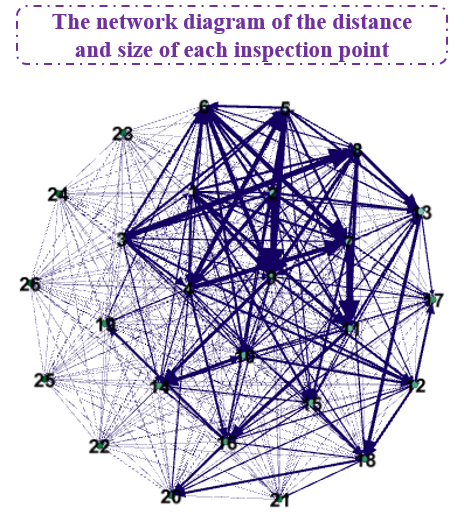
\includegraphics[height=10cm,width=12cm]{network}%图片名
	\caption{Global network}\label{fig:7}%题注
\end{figure}
Using the above two elements, we can describe this subnetwork after a simple observation. As for a example in figure2, the pop
$/$rock music occupies the largest area of the genre circle, indicating that it contains the largest number of artists. And the lines painted with its representative colors connect country music, folk music, blues music and so on, which means that rock music has a direct impact on these music. Among the lines from  pop$/$rock, the one which points to Blues music are obviously thicker than that points to light music, which shows that Pop$/$Rock music has more influence on the former than the latter.

\subsection{Influence Parameters}
For the purpose of quantifying the impact of each artist and better describing the influence network, we analyze the influence factors from three aspects: influence depth, influence speed and influence breadth.
\subsubsection{Influence Depth}
The depth of influence is to analysis the influence of artists vertically. With the classefication of genre, We can divide influence into two aspects as intra-class influence depth and inter-class influence depth.

\noindent%取消单段缩进
\textbf{Intra-class Influence Depth}

Intra-class Influence of Individual can measure the influence of an artist in a genre on others who are in the same genre. Its definition expression is as follows.
\begin{equation}
{I_{DA}} = \frac{{\sum\limits_j {{N_{{a_i} \to {a_j}}}} }}{{\sum\limits_i {\sum\limits_j {{N_{{a_i} \to {a_j}}}} } }}
\end{equation}
Where ${{N_{{a_i} \to {a_j}}}}$ represents the number of arrow from artist $i$ in genre $A$ to artist $j$ in the same genre.

\noindent%取消单段缩进
\textbf{Inter-class Influence Depth of Individual}

It is used to measure the influence of an artist in a genre on another genre, the expression of which is shown below.
\begin{equation}
I_{DR}^L = \frac{{\sum\limits_j {{N_{{a_i} \to {b_j}}}} }}{{\sum\limits_i {\sum\limits_j {{N_{{a_i} \to {b_j}}}} } }}
\end{equation}
Where ${{N_{{a_i} \to {b_j}}}}$ represents the number of line from artist $i$ in genre $A$ to artist $j$ in genre $B$. 

\noindent%取消单段缩进
\textbf{Inter-class Influence Depth of Genre}

It is the proportion of a genre’s influence on another genre in its influence on all genres. The difference between this parameter and the inter-class influence of individual is that it focuses on the influence of the genre rather than the influence of the individual on other genre. It can be expressed as the following equation.
\begin{equation}
I_{DR}^E = \frac{{\sum\limits_i {\sum\limits_j {{N_{{a_i} \to {b_j}}}} } }}{{\sum\limits_i {\sum\limits_j {{N_{{a_i} \to {b_j}}}}  + \sum\limits_i {\sum\limits_j {{N_{{a_i} \to {c_j}}}}  +  \cdots } } }}
\end{equation}
Where the denominator represents the total number of artists affected by a genre in other genres. In the global network, the higher the depth of influence between a genre and another one, the thicker the line connecting the two genres.



\subsubsection{Influence Speed}
Influence speed can quantitatively calculate how many years it takes for an artist to affect another artist. With the same method, the influence speed can be separated as intra-class influence speed and inter-class influence speed. 

\noindent%取消单段缩进
\textbf{Intra-class Influence Speed}

As a measure of how quickly an artist influences other artists within the genre, it can be defined as the equation here.
\begin{equation}
{I_{SA}} = \frac{{\sum\limits_j {({Y_{{a_j}}} - {Y_{{a_i}}})} }}{n_{1}}
\end{equation}
Where ${({Y_{{a_j}}} - {Y_{{a_i}}})}$ represents how many years it takes for artist $i$ in genre $A$ to influence artist $j$, and $n_{1}$ refers to the artists who are influenced by the artist $i$ in genre $A$.

\noindent%取消单段缩进
\textbf{Inter-class Influence Speed}

Based on the same principle, the inter-class influence speed shows as below.
\begin{equation}
{I_{SR}} = \frac{{\sum\limits_j {({Y_{{b_j}}} - {Y_{{a_i}}})} }}{n_{2}}
\end{equation}
Where ${({Y_{{a_j}}} - {Y_{{a_i}}})}$ represents how many years it takes for artist $i$ in genre $A$ to influence artist $j$ in genre $B$, and $n_{2}$ refers to the number of artists who are influenced by the artist $i$ in genre $B$.

\subsubsection{Influence Breadth}
As a horizontal measure, influence breadth can be defined as the total number of categories influenced by an indivudal artist.
\begin{equation}
{I_B} = {N_{{a_i} \to X}}
\end{equation}
Where ${N_{{a_i} \to X}}$ is the notation of the number of genres influenced by artist ${{a_i}}$.



\subsection{Subnetwork}
The global network map reflects the complex relationship of influence and influence among all artists. However, it is difficult to intuitively observe the influence of a certain artist in a certain music genre on other genres. Therefore, We extract a subnetwork from the global network to describe this impact. Aim to express and analyze subnetwork more concisely, all artists are divided into the following three categories.
\begin{itemize}
	\item Artists who only influence others.
	\item Artists who influence some people and are also influenced by others.
	\item Artists who are only influenced by others.
\end{itemize}
With the artists classification, to express the subnetwork more clearly, we select a representative part of it and present here.
\begin{figure}[H]%图片
	\small
	\centering
	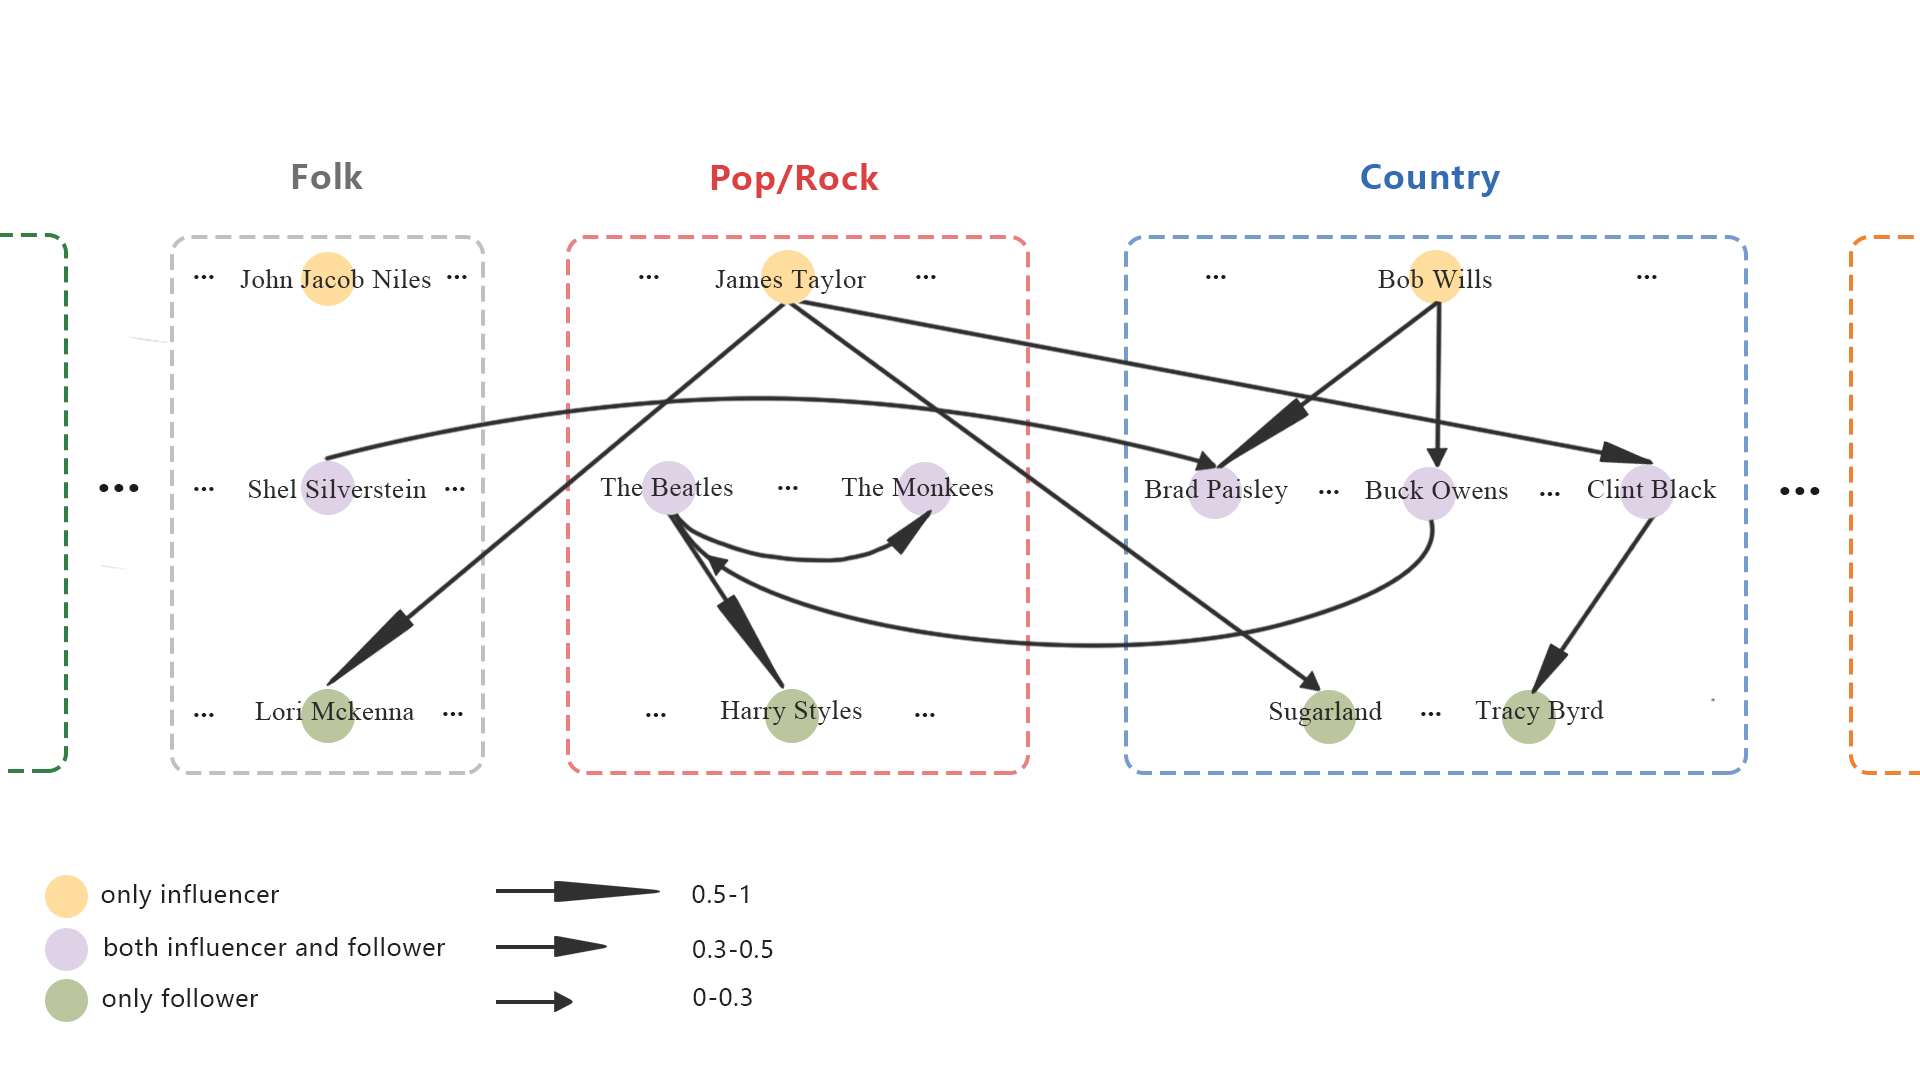
\includegraphics[height=9cm,width=14cm]{subnetwork}%图片名
	\caption{subnetwork}\label{fig:7}%题注
\end{figure}
In the above figure, three different colors are used to express the three kinds of artists above, while the arrows point from influencers to followers. The intra-class and inter-class influence depth of individual is shown in the figure as the proportion of arrows pointing from an artist to his or her genre and to other genres. And influence speed within and between classes is expressed as the arrow shapes. As for the influence breadth, it is the number of arrows from one artist to another genre.

\section{Similarity Comprehensive Evaluation Model}
The similarity between artists is a profile of their mutual influence, which makes it very valuable for investigating the results of influence.In the model, we use factor analysis to reduce the dimension of parameters and apply the weight to the calculation of modified cosine similarity, which is a overall index to quantify the similarity.

\subsection{Factor Analysis}
Since too many variables will hinder the establishment of the search law, we must first reduce the dimensionality of plent of  parameters provided by the file. To confront this problem, We use factor analysis[2] to determine comprehensive evaluation indicators.

In order to verify the applicability of the factor analysis method to the selected data, the KMO test is first performed on the data. And the test statistic is 0.630>0.5, indicating that the selected data has a strong correlation; Secondly, the Bartlett spherical test is performed, and the test statistic is 0 <0.05. The results show that the selected data are in a spherical distribution, which meets the conditions of use of factor analysis.

Through the data analysis of SPSS, the common factors are generated, and the subordinate relationship between them is determined according to the correlation coefficient between the parameters and the common factors. The final weight of each parameter and common factor is shown in the figure below.
\begin{figure}[H]%图片
	\small
	\centering
	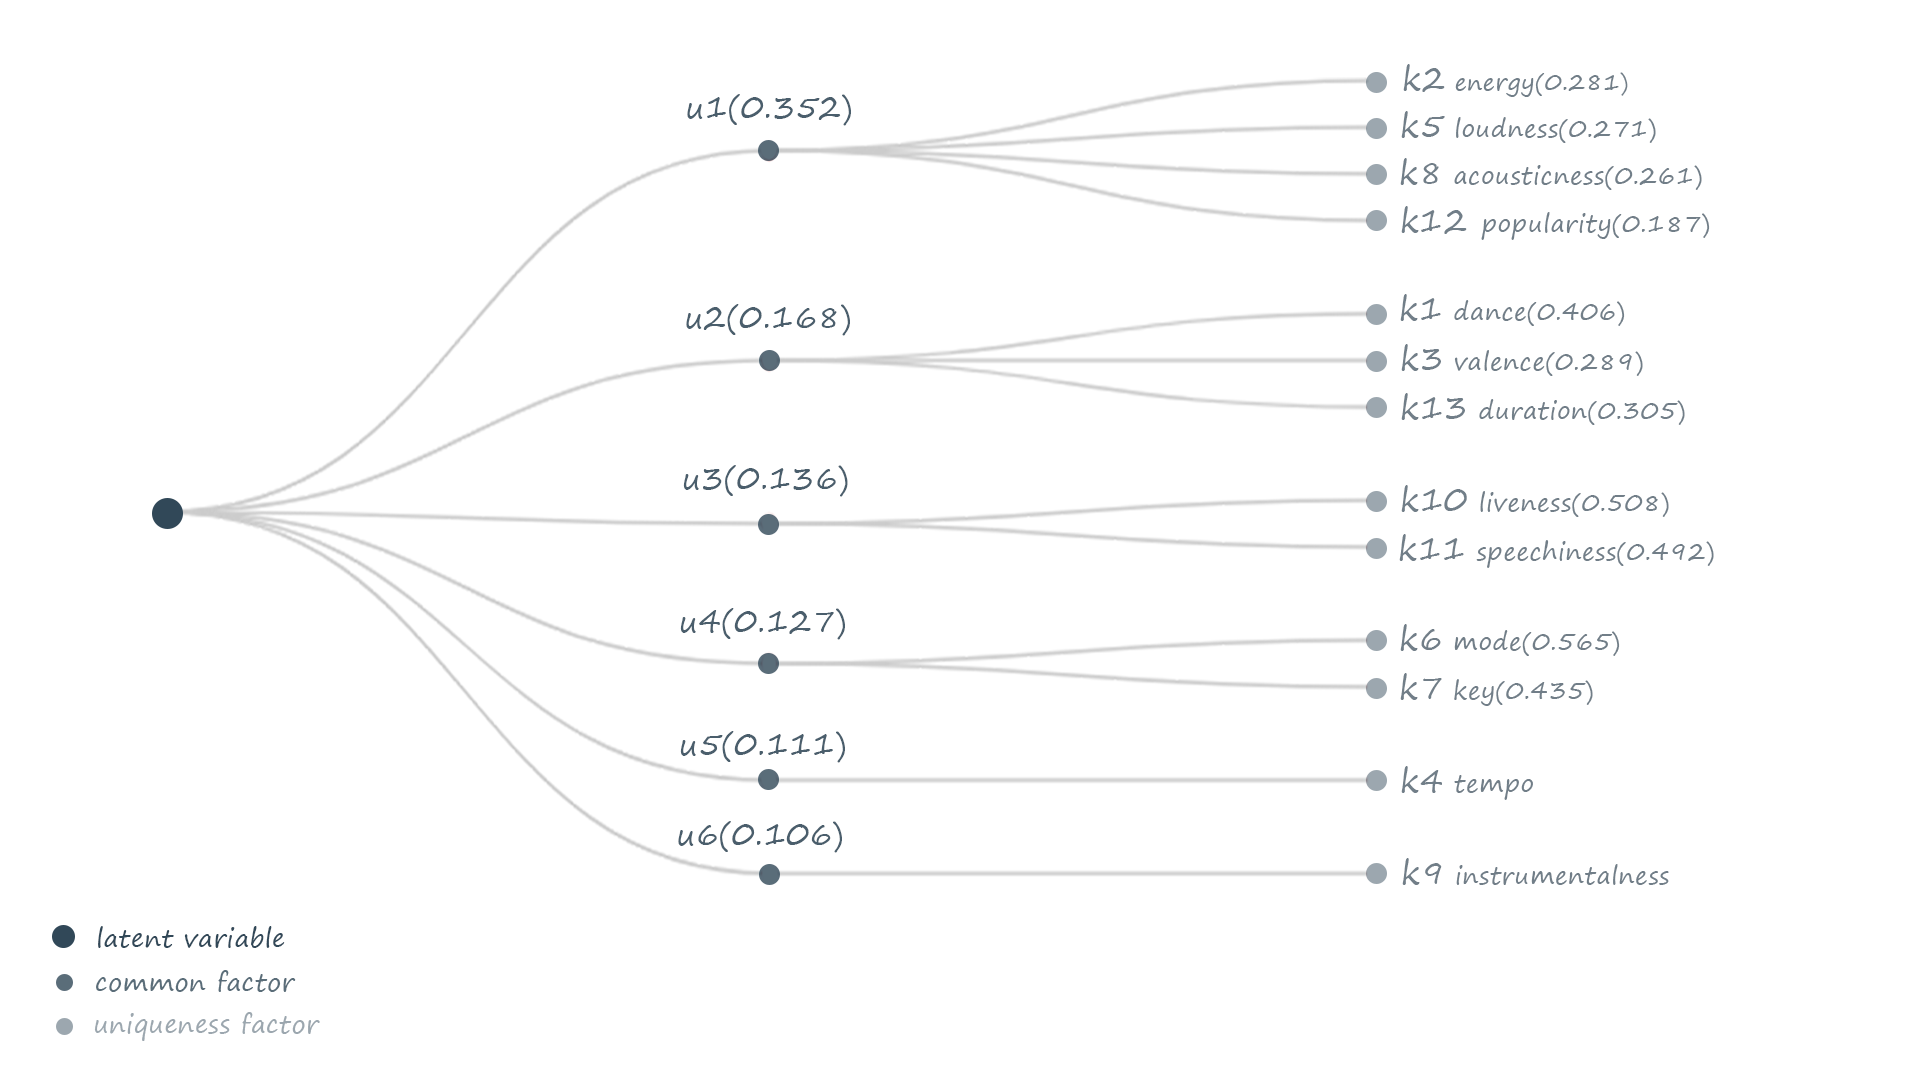
\includegraphics[width=14cm]{factor analysis}%图片名
	\caption{Factor weight}\label{fig:7}%题注
\end{figure}
Based on the above analysis, the provided parameters are reduced into six common factors, but an overall index is still needed to quantify the similarity, which will be described in detail in next section.
\subsection{Modified Cosine Similarity}
There are many methods for comparing the similarity of data, such as Euclidean distance, cosine similarity and Pearson correlation coefficient. However, Euclidean distance cannot deal with indicators of different importance, while cosine similarity does not take into account the problem of scoring scale, and the Pearson correlation coefficient ignores the differences of scoring schemes of different users.

To combine the advantages of the above methods and avoid the disadvantages, modified cosine distance[1] is selected as the overall index to measure the similarity of artists. Its expression is shown as follows.
\begin{equation}
dsim(i,j) = \frac{{\sum\nolimits_{k = 1}^6 {({U_{k,i}} - } {{\bar U}_k})({U_{k,j}} - {{\bar U}_k}){W_k}}}{{\sqrt {\sum\nolimits_{k = 1}^6 {({U_{k,i}} - } {{\bar U}_k}){W_k}^2} \sqrt {\sum\nolimits_{k = 1}^6 {({U_{k,j}} - } {{\bar U}_k}){W_k}^2} }}
\end{equation}
Where the ${{U_{k,i}}}$ and ${{U_{k,j}}}$ represents the $k$-th common factor of artist $i$ and artist $j$, ${{{\bar U}_k}}$ means the average of the $k$-th common factor, and ${{W_k}}$
is the notation of the weight calculated in Section 4.1. According to equation 6, the smaller the modified cosine similarity is, the more similar the two artists are. In that case, We take the reciprocal of it as the modified cosine similarity to facilitate the following description.
\begin{equation}
sim(i,j) = \frac{1}{{dsim(i,j)}}
\end{equation}

On the basis of the above formula, we can calculate the modified cosine similarity between each artist and other artists one by one. With the same idea as the parameter definition in the first question, define two similarity indicators between and within genres.

\noindent%取消单段缩进
\textbf{Intra-class Similarity}

Intra-class similarity is the average of similarity among all artists in a genre, which can be expressed as below.
\begin{equation}
{S_{MM}} = \frac{{\sum\limits_i {\sum\limits_j {sim(i,j)} } }}{{{n_1}}}{\rm{       (}}i,j \in M,i \ne j)
\end{equation}
Where $n_{1}$ is the number of the modified cosine similarity
in genre $M$.

\noindent%取消单段缩进
\textbf{Inter-class Similarity}

Inter-class similarity is the average value of similarity between all artists in one genre and all the ones in another genre.
\begin{equation}
{S_{MN}} = \frac{{\sum\limits_i {\sum\limits_j {sim(i,j)} } }}{{{n_2}}}{\rm{       (}}i \in M,j \in N,i \ne j)
\end{equation}
Where $n_{2}$ is the number of the modified cosine similarity
between the artists of genre $M$ and $N$.

Based on the above two similarity indicators, we can create a 20 by 20 similarity matrix as follows.
\begin{equation}
S = \left( {\begin{array}{*{20}{c}}
	{{S_{11}}}& \ldots &{{S_{1,20}}}\\
	\vdots & \ddots & \vdots \\
	{{S_{20,1}}}& \cdots &{{S_{20,20}}}
	\end{array}} \right)
\end{equation}

 In accordance with the matrix above, select the five genres that are most similar to each genre and list them in each row of Table 2. For brevity, part of the genres are shown. The similarity level in the first row of the table corresponds to the five largest numbers in each row of the matrix. The higher the level, the higher the similarity between the two genres. And if a genre has the highest degree of similarity to itself, which means that the similarity within the genre exceeds that between genres. 
\begin{table}[H]
	\centering  
	\caption{Similarity degree table}
	
	\label{table_time}
	
	\begin{tabular}{cccccc}  
		
		\toprule   
		
		Genre&4 &3&2&1&0\\ 
		
		\midrule   
		Classical&Classical&Easy Listening&Stage $\&$ Screen&Vocal&Jazz \\ 
		Country&Country&Children's &Religious&Folk&Pop $/$ Rock
		\\  
		Electronic & Country&Pop $/$ Rock & Blues&Children's&R$\&$B
		\\    
		Jazz &Easy Listening&Jazz& Folk&Pop $/$ Rock&Blues
		\\
		Children's&Children's&Country&Religious&Folk&Pop $/$ Rock
		\\
		\bottomrule  
		
	\end{tabular}
\end{table}
Observing the above table, we can draw the following conclusions.
\begin{itemize}
	\item For some genres, artists within which are more similar than those between genres such as Classical, Country, Children's.
	\item For some genres, artists between genres are more similar than those within genres such as Jazz and Electronic music. After analyzing the data in detail, we believe that this is because these genres tend to have strong horizontal expansion and can quickly develop works with different styles under the same genre spirit. For example, Electronic music uses the keyboard to simulate various sound effects and even produces effects that cannot be achieved by real instruments, which determines that it can develop into different music styles, melody, tunes, etc. Thus, it is not difficult to understand that the similarity of musicians within this genre is even lower than that between genres.
\end{itemize}

To further prove this point, it is also necessary to perform a significant test on the intra-class similarity and the inter-class similarity. Taking into account that the actual similarity values are not normally distributed, the non-parametric[3] test is selected, and the significance level sig of them is 0. The consequence fully shows that the similarity between the artists in the same genre and the similarity between  the ones in diverse genre are significantly different, which proves our conclusion from another point of view.

\section{Genre Distinction}
\subsection{Comparison of Similarities $\&$ Influence}

\noindent%取消单段缩进
\textbf{Comparison of Similarities} 

In order to compare the similarity between genres quantitatively, we use equation 10 to calculate the similarity between classes. Taking into account the representativeness of the data, We only list the three highest values and the three lowest values.
\begin{table}[H]
	\centering  
	\caption{Inter-class Similarity Ranking}
	
	\label{table_time}
	
	\begin{tabular}{cccc}  
		
		\toprule   
		
		Genre&Genre &Inter-class similarity&Rank \\ 
		\midrule    
		Country&Children's&1.12525&1
		\\  
		Comedy$/$Spoken&Pop$/$Rock & 1.05125&2 
		\\ 
		Country &R$\&$B& 1.04166&3
		\\
		Reggae&New age&0.46232&188
		\\
		Comedy$/$Spoken&Avant-Garde&0.42063&189
		\\
			Comedy$/$Spoken&New age&0.38180&190
		\\
		\bottomrule  
	\end{tabular}
\end{table}
From the above table, among the 20 genres, country music and children’s music are the most similar, while Comedy$/$Spoken and New age music are the least similar.


 For the sake of comparing the similarities within genres, we sort the in-class similarity of genres as shown in the following table. 
\begin{table}[H]
	\centering  
	\caption{Intra-class Similarity Ranking}
	
	\label{table_time}
	
	\begin{tabular}{ccc}  
		
		\toprule   
		
		Genre& Intra-class similarity&Rank \\ 
		\midrule    
		Country&1.308874&1
		\\  
		Religious & 1.046841&2 
		\\ 
		Folk & 1.041238&3
		\\       
		Electronic &0.686901&18
		\\
		Comedy$/$Spoken&0.619346&19
		\\
		Avant-Garde&0.60525&20
		\\
		\bottomrule  
		
	\end{tabular}
\end{table}
It can be seen from the above table that Country music has the highest degree of inter-class similarity, indicating that this genre is more stable and uniform. On the contrary, the Avant-Garde music has the lowest degree of inter-class similarity, reflecting its large internal variability, strong expansion, and large free creation space.



\noindent%取消单段缩进
\textbf{Comparison of Influence} 

 To compare the influence between genres, use the inter-class influence depth of genre in section 3.2 to measure it, and a part of the data is as follows.
 \begin{table}[H]
 	\centering  
 	\caption{Influence between genres}
 	
 	\label{table_time}
 	
 	\begin{tabular}{ccc}  
 		
 		\toprule   
 		
Genre&Affected Genre &Inter-class influence depth of genre \\ 
 	\midrule   
 		Avant-Grade & Classical &0.0632911 \\
 		Avant-Grade & Electronic &0.2151899    \\ 
 		Blues&Country&0.004827  \\    
 		
 		\bottomrule  
 		
 	\end{tabular}
 \end{table}
According to the data in Table 4, Avant-Garde music has a greater impact on Electronic music, while Blues has a smaller influence on Country music.

As for the influence within the genre, the intra-class influence  is used to quantify it, the data of Avant-Grade is shown below.
\begin{table}[H]
	\centering  
	\caption{Influence between genres}
	
	\label{table_time}
	
	\begin{tabular}{ccc}  
		
		\toprule   
		
		Artist name&\quad &Intra-class influence \\ 
		
		\midrule   
		Harold Budd&\quad &0.14286 \\
		Moondog&\quad&0.285714286
		    \\  
		
		Terry Riley& \quad&  0.428571429
		\\    
		
		Meredith Anderson&\quad& 0.142857143
		 \\
		
		\bottomrule  
		
	\end{tabular}
\end{table}
  We can find out intuitively from the above table that in Avant-Garde music, Harold Budi has the most influence, while Meredith Anderson has less influence.
 \subsection{Distinguishing Indicators}

 
 In the light of the large number of indicators provided by the given file, we need to determine the indicators that can best distinguish each genre. 
 
 Through the statistical analysis of a large number of music characteristics data through SPSS software, it is found that it basically conforms to the normal distribution. To compare the differences of music characteristic among music genres, we need to carry out significance analysis. Considering that this is the significance test of the same factor among multiple groups of categories, we can not carry out independent sample t-test. In that case, duncan method is chosen to confront this problem.
 \begin{table}[H]
 	\centering  
 	\caption{Average significance level ranking}
 	
 	\label{table_time}
 	
 	\begin{tabular}{ccc}  
 		
 		\toprule   
 		
 		Characteristic&Average Significance level &Rank \\ 
 		\midrule    
 		speechiness&0.00195&1
 		\\  
 		instrumentalness & 0.00979&2 
 		\\ 
 		Acousticness & 0.01075&3
 		\\       
 		Mode &0.05466&13
 		\\
 		Key&0.10180&14
 		\\
 		Tempo&0.505173&15
 		\\
 		\bottomrule  
 		
 	\end{tabular}
 \end{table}
 Observing the above table, we can see that the significance level of speech and musical instruments is lower than 0.01, indicating that the data differences under these two characteristics are very significant. According to the principle mentioned above,  the greater the difference, the better the distinguishing effect. So the speechiness
  and instrumentalness are the most suitable indicators for distinguishing.


\subsection{Change of the Genre} 
 
 In order to get the trend of each music genre over time, first use the code to match the musicians in the full$\_$music$\_$data file with the corresponding music genre; Second, according to the music genres, all the data are grouped into 16 categories. Lastly, the data visualization is carried out by using the data perspective toolbox of Excel to get the change of the average annual value of each music characteristics over time. 
 
 To illustrate the trend of music characteristics over time, we choose song circulation as examples and draw their time series as shown here. To get the data of the song circulation, We first divide the music into 20 categories according to the genres, and then use data perspective to analyze the individual factions, finally calculate the number of songs released in each year.
 \begin{figure}[H]%图片
 	\small
 	\centering
 	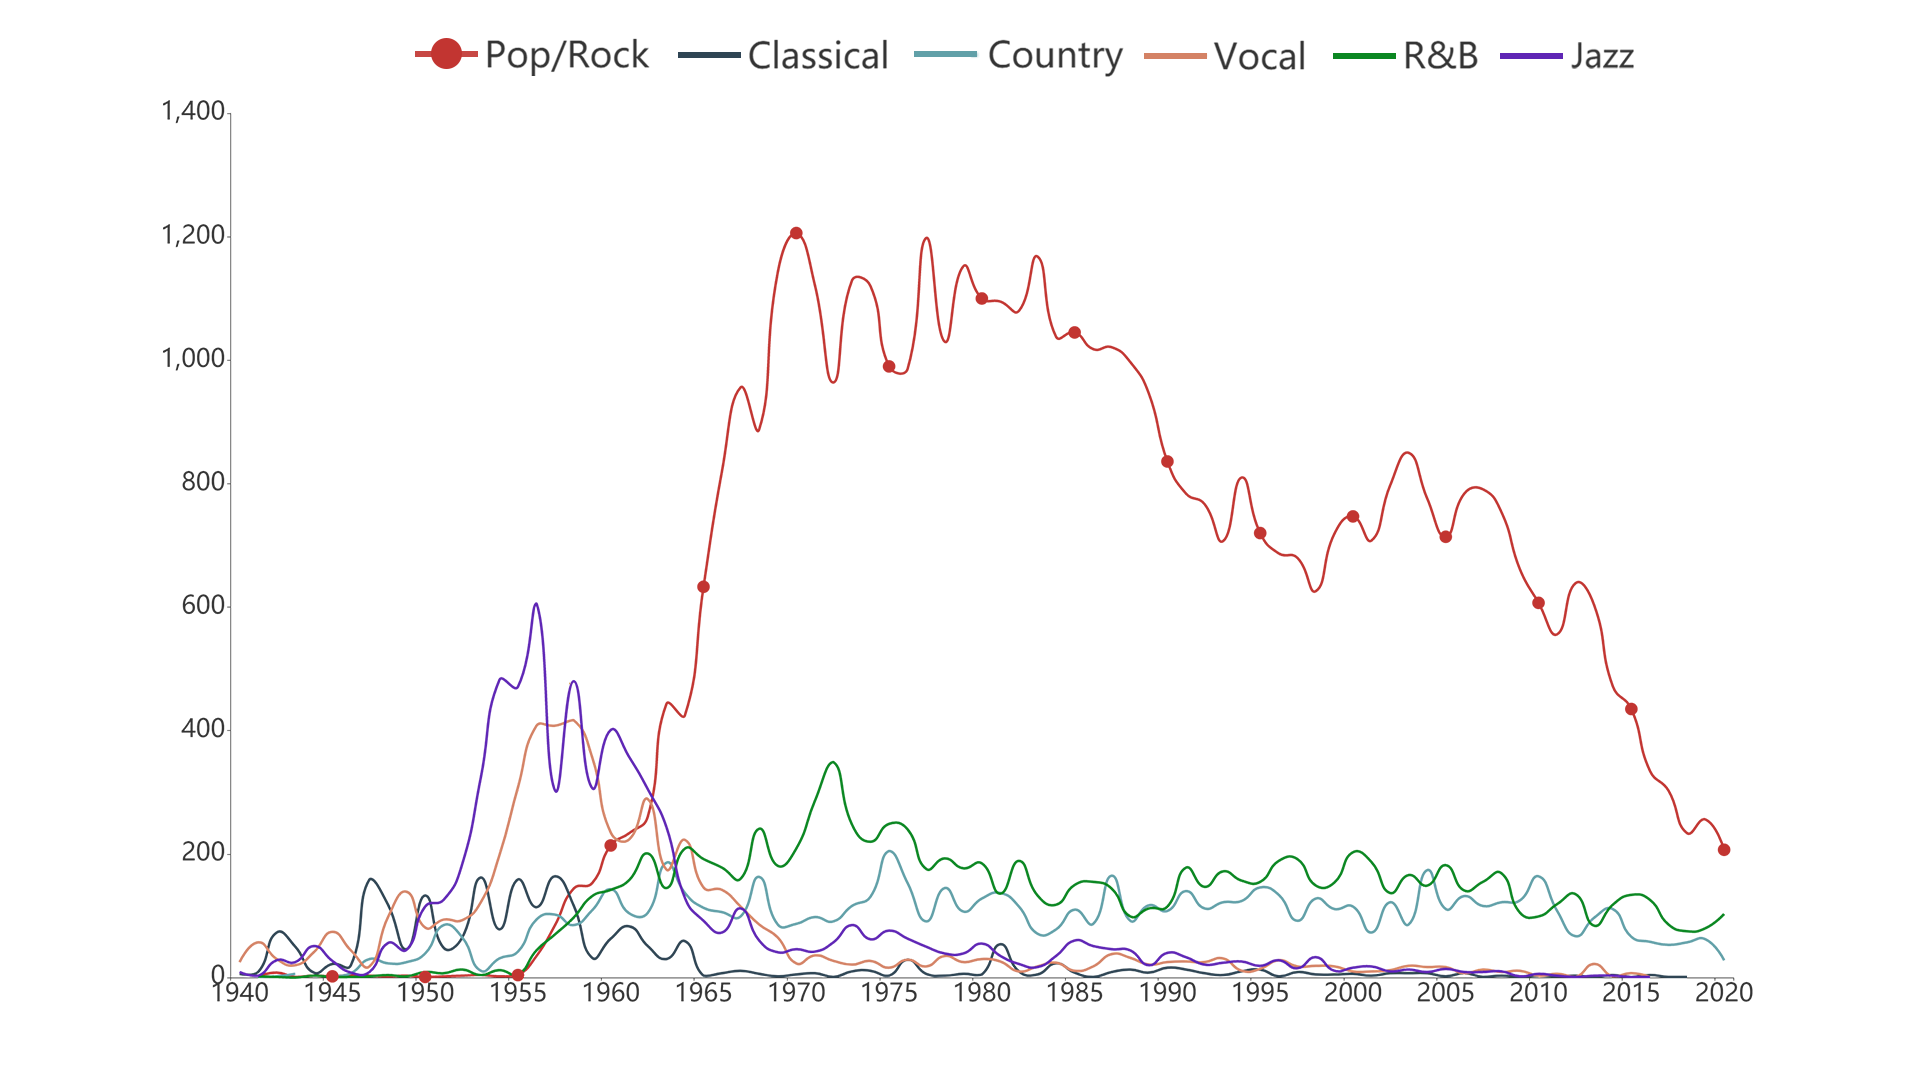
\includegraphics[height=9cm,width=14cm]{ccl}%图片名
 	\caption{Song circulation}\label{fig:7}%题注
 \end{figure}
 From the above table, we can draw the following conclusions.
 \begin{itemize}
 	\item After 1945, the circulation of Classical music rose first and occupied the main market in the next three years. After that, the circulation fluctuated slightly until it declined rapidly in the middle and late 1960s.
 	\item After 1948, the circulation of Classical music was surpassed by Jazz and Vocal music, the latter two peaked in the 1950s and early 1960s, and decreased significantly after the rise of Pop $/$Rock music;
 	\item In the late 1960s, Pop$/$Rock music became the number one in the circulation list, and its circulation has been the champion from the 1970s to today. 
 \end{itemize}
\subsection{Relationship Between Genres}
 In line with the comparison of similarity between genres in Section 5.1, we can find out that the similarity between Country music and Children's music, Comedy$/$Spoken music and Pop$/$Rock music, Country music and R$\&$B music are much higher than others, whihc shows that they are closely related.
\section{Exploration of Actual Influence}
\subsection{Real Affect of Influencers}
For further study about whether the influencer can really affect the followers, we only calculate the modified cosine similarity between the artists with influence and affected relationship, and then reconstruct the similarity matrix based on this.

With the same method as the second question to reduce the dimensionality of the data to obtain six common factors, calculate the similarity between the artists with influence relationship according to equations 7 and 8, and then use equations 9 and 10 to get the new intra-class and inter-class similarity, which represented by $S_{MM}^{'}$ and $S_{MN}^{'}$. Based on the above process, we can get a new similarity matrix as follows.
\begin{equation}
S^{'} = \left( {\begin{array}{*{20}{c}}
	{S_{1,1}^{'}}& \ldots &{S_{1,20}^{'}}\\
	\vdots & \ddots & \vdots \\
	{S_{20,1}^{'}}& \cdots &{S_{20,20}^{'}}
	\end{array}} \right)
\end{equation}

Using the above formula and the similarity matrix in the second question, the growth rate of similarity between genre $M$ and genre $N$ can be derived as below.
\begin{equation}
G_{MN} = \frac{{S_{MN}^{'} - {S_{MN}}}}{{{S_{MN}}}}
\end{equation}
Therefore, the average growth rate of similarity is
as shwon here.
\begin{equation}
G^A = \frac{{\sum {{G_{MN}}} }}{{{n_{i \to f}}}}
\end{equation}
Where the genre $M$ and genre $N$ have direct realtionship of influence and the ${{n_{inf \to flo}}}$ represents the number of the ${{G_{MN}}}$.

And the average of intra-class influence and inter-class influence is defeined as follows.
\begin{spacing}{1.2}
\large
\begin{equation}
\left\{ \begin{array}{l}
G_{MM}^A = \frac{{\sum {{G_{MM}}} }}{{n_{_{i \to f}}^{tra}}}\\
G_{MN}^A = \frac{{\sum {{G_{MN}}} }}{{n_{_{i \to f}}^{ter}}}(M \ne N)
\end{array} \right.
\end{equation}
\end{spacing}
Substituting the data into the above expression can obtain the values of the above three parameters as shown in the following table.
\begin{table}[H]
	\centering  
	\caption{Similarity growth rate}
	
	\label{table_time}
	
	\begin{tabular}{ccc}  
		
		\toprule   
		
		Parameter&Value($\%$) \\ 
		
		\midrule   
		Average similarity growth rate&20.37411597
		\\
		Average intra-class similarity growth rate &20.08829769
		\\  
		
		Average inter-class similarity growth rate& 21.30866782
		\\  
		
		\bottomrule  
		
	\end{tabular}
\end{table}
It can be concluded from the above table that in the case of only influencers and followers, the similarity has been improved to a certain extent, indicating that influencers really have an impact on the creation of followers.
\subsection{‘Contagious’ Characteristics}
Aim to quantify the infectivity of each characteristic, we subtract the data of 20 genres corresponding to each characteristic and take the absolute value as an index to measure the similarity. Considering that the number of artists affected by each genre is different, the final growth rate expression needs to add weights. So the growth rate of average similarity between genre $M$ and genre $N$ can be defined as following.
\vspace{-0.35cm} %设置与上面正文的距离
\begin{spacing}{1.4}
	\large
\begin{equation}
\left\{ \begin{array}{l}
{G^A} = \frac{{\sum {{G_{MN}}{W_{MN}}} }}{{{n_{i \to f}}}}\\
G_{MM}^A = \frac{{\sum {{G_{MM}}} }}{{n_{_{i \to f}}^{Intra}}}\\
G_{MN}^A = \frac{{\sum {{G_{MN}}} }}{{n_{_{i \to f}}^{Inter}}}(M \ne N)\\
{W_{MN}} = \frac{{{n_{M \to N}}}}{{{n_{i \to f}}}}
\end{array} \right.
\end{equation}
\end{spacing}
\vspace{-0.35cm} %设置与上面正文的距离
Where the ${{n_{M \to N}}}$ represents the number of the arrow from genre $M$ to genre $N$ and ${{n_{i \to f}}}$ refers to the number of arrows from genre $M$ to other genres.

In accordance with the above expression, the similarity growth rate can be obtained here. Since mode and key are a series of discrete variables, it is not meaningful to find their similarity growth rate, so only the values of the remaining continuous characteristics are calculated.
\begin{table}[H]
	\centering  
	\caption{Similarity growth rate of characteristic}
	
	\label{table_time}
	
	\begin{tabular}{cccc}  
		
		\toprule   
		
		Characteristic&${G^A}$($\%$) &$G_{MM}^A$($\%$)&$G_{MN}^A$($\%$) \\ 
		\midrule    
		danceability&29.244387&29.71417491
		&27.70830198
		\\  
		acousticness&17.1484511&17.21497367
		&16.93093949
		\\ 
		energy& 16.96905204
		&16.70750978&17.8242275\\
		tempo&	16.87008699&	16.26035567	&18.86375075
		\\      
		valence	&16.18718803&	16.461186&	15.29128552
		 \\
		 popularity	&13.57494464&	13.36014218&	14.27729314
		 \\
		 loudness&	11.42854953&	10.80444531&	13.46920894
		 \\
		 duration$\_$ms&	10.6711244&	10.97337902&	9.682829939
		 \\
		 liveness&	9.73555416&	9.889043085&	9.23368506
		 \\
		 instrumentalness&	8.70029275&	6.832079709&	14.80886635
		 \\
		\bottomrule  
		
	\end{tabular}
\end{table}
Analyzing the data in the above table, we can see that when only considering genres with influential relationships, the growth rate of the similarity of danceability is the largest compared to when all genres are considered. It indicates that danceability is the most ‘contagious’ characteristic.
\section{Revolution of Music Genres}
\subsection{Determination of characteristics}
 To find out the characteristics that marked a significant leap in music evolution, we combined with the data obtained through data perspective from the third question. By analyzing the time series of each characteristic of the 20 music genres, we can find them with obvious jump trend, and then record the corresponding time nodes, so as to determine the corresponding characteristics of the changes of each music genre. 
 By traversing the changes of each characteristic on the time axis, the following rules can be found.
 \begin{itemize}
 	\item The jump point of each music characteristic of Pop/Rock and R$\&$B were basically concentrated in 1955, and the difference sequence diagrams of all characteristic became very stable after that.
 	\item The jump point of popularity is mainly concentrated between 1945 and 1955. Before that, the numerical fluctuation is large or the numerical value is too small, which shows that it has not been widely accepted by the public. However, the popularity of various music genres began to grow rapidly after 1955.
 	\item The circulation of songs keeps pace with the growth of popularity. The jump point of Jazz, Vocal and Classic is about 1945, while Pop$/$Rock, R$\&$B and Country's appeared in 1955.
 	\item As for the Easy Listening, it showed the same trend after 1970.
 	\item The jump point of Avant-Garde was 1960. Before that, the four musical properties of duration$\_$ms, key, loudness, acousticness, and instrumentalness all changed smoothly over time, but after that, their volatility began to increase. 
 	
 
 Due to the large number of time series diagrams, we only show two of them as follows.
 \end{itemize}
\begin{figure}[H] %这里使用的是强制位置,除非真的放不下,不然就是写在哪里图就放在哪里,不会乱动
	\centering  %图片全局居中
	\vspace{-0.35cm} %设置与上面正文的距离
	\subfigtopskip=2pt %设置子图与上面正文或别的内容的距离
	\subfigbottomskip=2pt %设置第二行子图与第一行子图的距离,即下面的头与上面的脚的距离
	\subfigcapskip=5pt %设置子图与子标题之间的距离
	\subfigure[Change of Popularity]{
		\label{level.sub.1}
		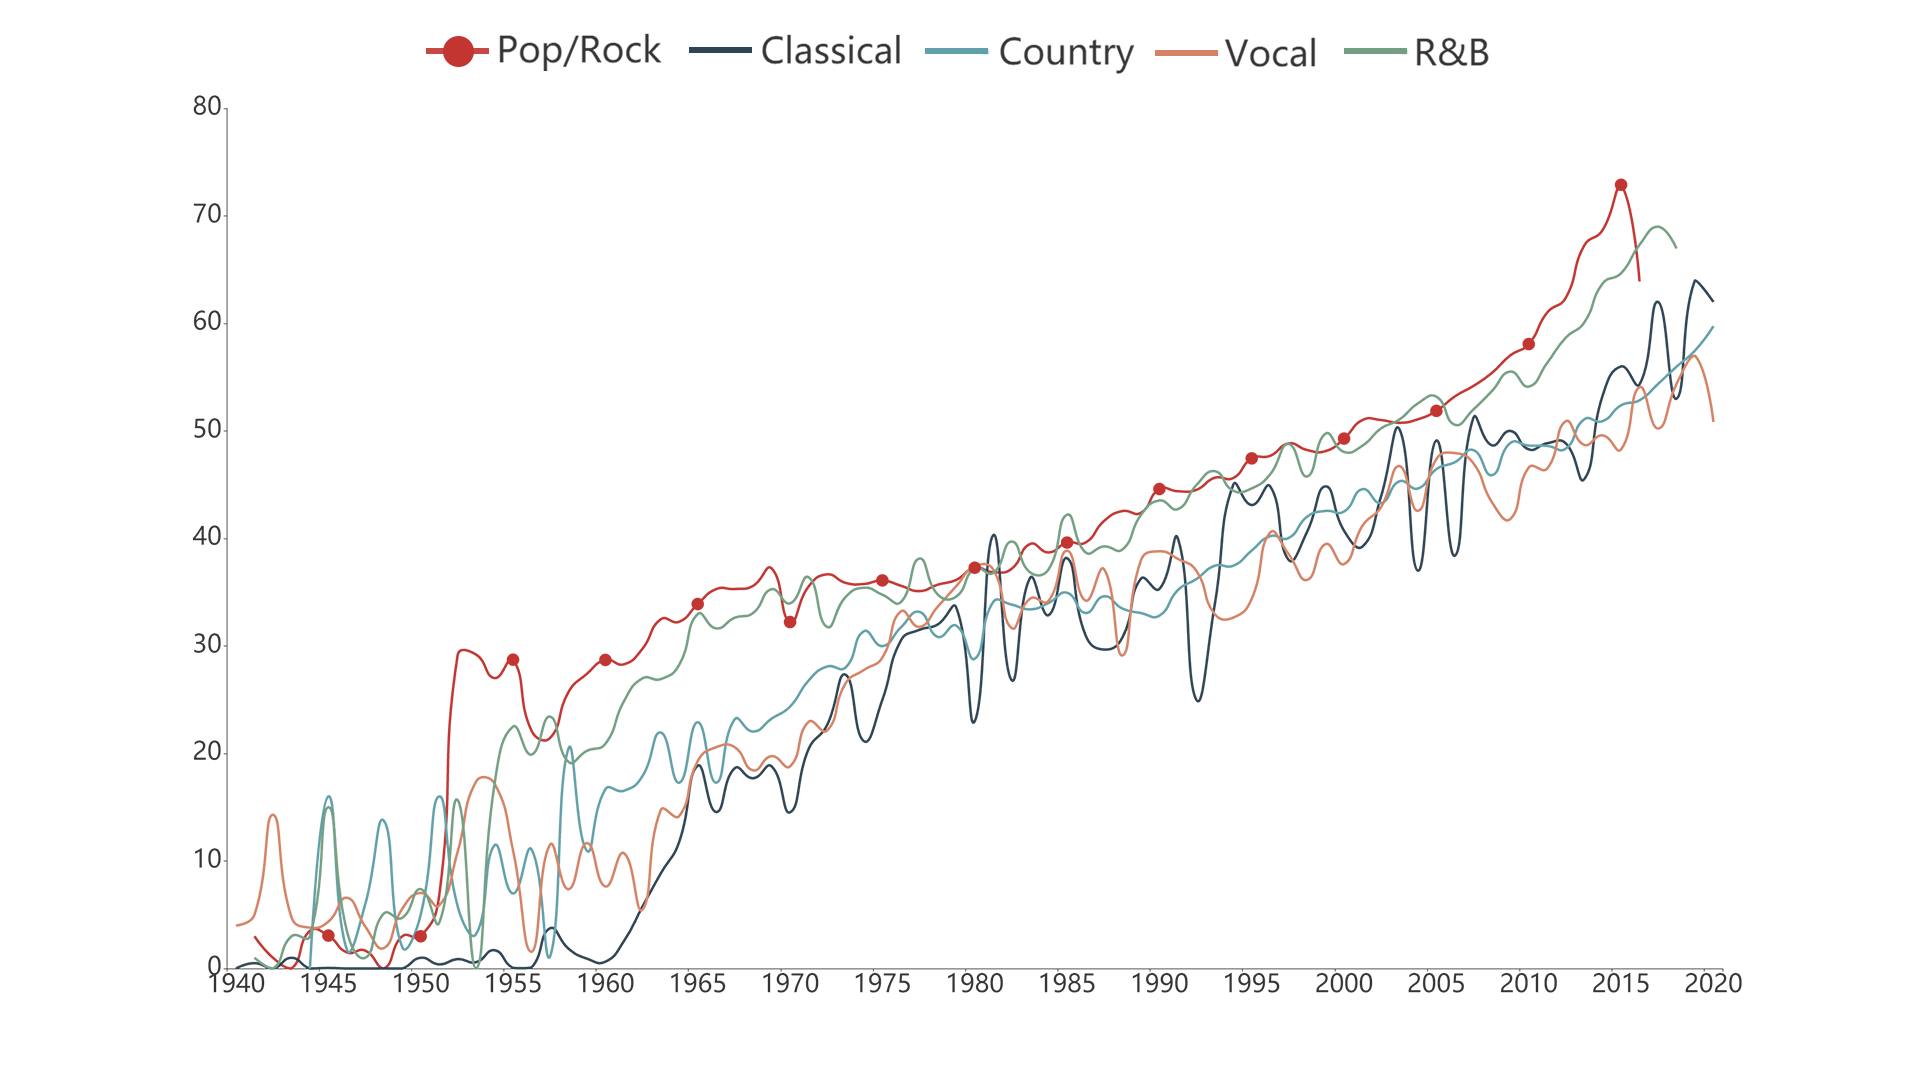
\includegraphics[height=6cm,width=7.8cm]{popularity}}
	\quad %默认情况下两个子图之间空的较少,使用这个命令加大宽度
	\subfigure[Change of the Characteristics of R$\&$B]{
		\label{level.sub.2}
		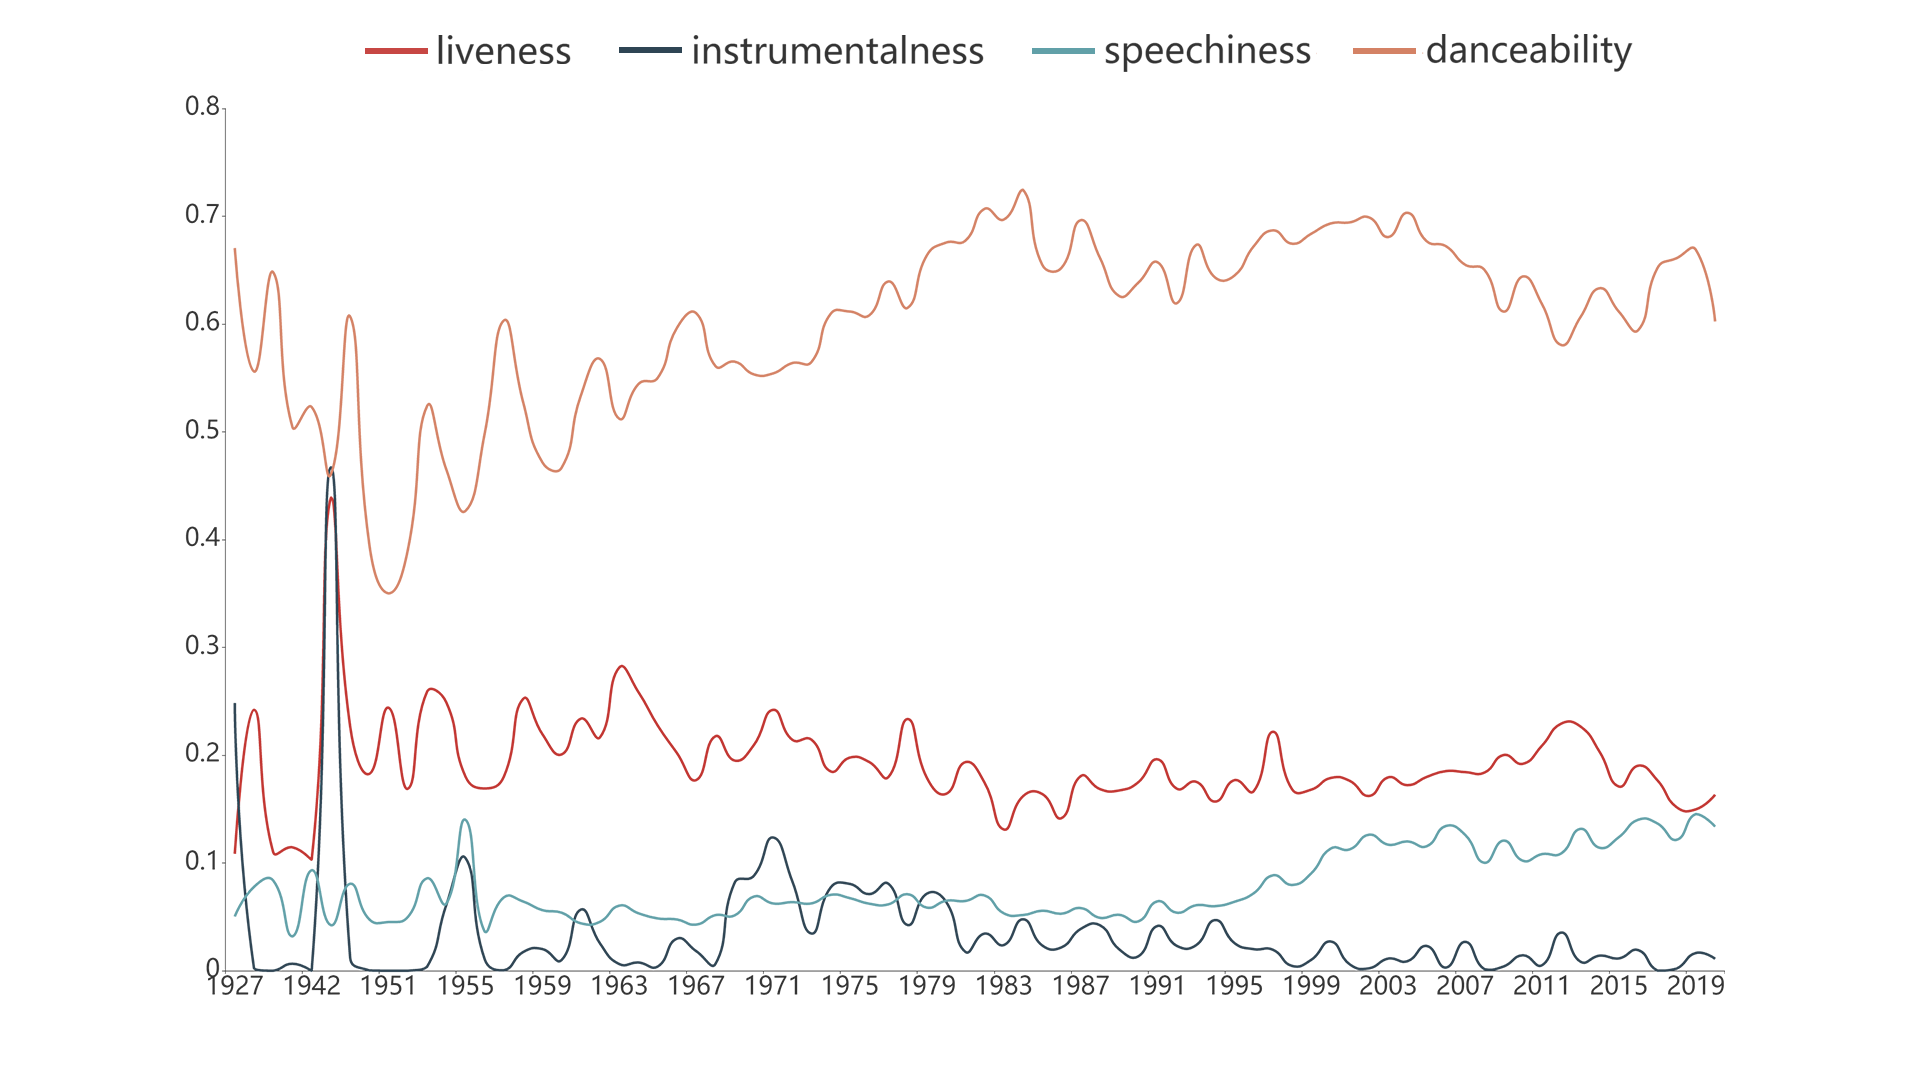
\includegraphics[height=6cm,width=7.8cm]{RB}}
	\caption{Time series diagrams}
	\label{level}
\end{figure}
\subsection{Determination of Revolutionaries}
The revolutionary of music should have opened an era of music represented by him. This era has distinct characteristics that are different from the previous ones, and the revolutionary has an important influence on his followers in these characteristics. In that case, combining the analysis of the jump points in Section 7.1, revolutionaries are most likely to appear near the jump points of specific characteristics.

Aim to identify the revolutionaries, we first analyze the time series diagrams of each music characteristic, and find out the music genres that have a jump at the same point for a certain characteristic. And according to the trend after the jump, divide them into some similar sets, thus narrowing the scope of the revolutionary selection. Some data are shown in the following table.
\begin{table}[H]
	\centering  
	\caption{Jump Year and Trend Division}
	
	\label{table_time}
	
	\begin{tabular}{ccccc}  
		
		\toprule   
		
		Characteristic&Jump year&Rising&Decling&Fluctuating \\ 
		\midrule    
		Popularity&1945$\sim$1955&All of the genres&n$/$a&n$/$a
		\\  
		Song circulation&1955&Pop$\&$Rock,R$\&$B&Folk,Vocal&Classical
		\\ 
		Acousticness&1950$\sim$1960&n$/$a&Country,R$\&$B&Easy Listening\\
		Duration$\_$ms&1960$\sim$1970&Pop$\&$Rock,R$\&$B&n$/$a	&Vocal,Avant-Garde
		\\      
		\bottomrule  
	\end{tabular}
\end{table}
Where rising, decling and fluctuating indicates the trend after a jump, while the n$/$a means not applicable. 

According to the previous analysis, the characteristics of revolutionaries are consistent with the trend of the genres influenced by revolutionaries near the jump point, so we can find the influencers who meet this requirement in the genres contained in the similar sets. At the same time, considering the order of influence and being affected, the active start time of revolutionaries must be earlier than the jump point.

On the basis of the above analysis, choose suitable influencers, and then select the part contained in the same similar set from its corresponding followers. In order to find the follower who is more affected, calculate the similarity between this part of the follower and the influencer according to Equation 8, and normalize it. The threshold is set to 0.5, and followers above the threshold are called effective followers. Count the number of effective followers corresponding to each qualified influencer, and use this as the main criterion to measure revolutionaries. Finally, choose the top five artists with the most effective followers as revolutionaries, which is shown as below.
\begin{table}[H]
	\centering  
	\caption{List of Possible Revolutionaries}
	
	\label{table_time}
	
	\begin{tabular}{cccc}  
		
		\toprule   
		
		Artist&Genre &Time&Valid mumber of follower \\ 
		\midrule    
		The Beatles&Pop$\&$Rock&1960&455
		\\  
		Bob Dylan&Pop$\&$Rock&1960
		&264
		\\ 
		Hank Williams&Country
		&1930&132\\
		Marvin Gaye&R$\&$B&	1950	&121
		\\      
		Miles Davis	&Jazz&	1940&	116
		\\
		\bottomrule  
		
	\end{tabular}
\end{table}
In the light of results in the above table, the Beatles and Bob Dylan are more likely to be called revolutionaries.

\section{Dynamic Influence}
 With many music genres at their peak, Pop/Rock can climb rapidly in a short period of time with its amazing speed, successfully defeating all opponents and becoming the top stream in the music industry. There must be powerful dynamic influencers behind it. Therefore, in this section, we mainly discuss the dynamic influence process of Pop/Rock in music innovation.
 
  To find out the indicators that reveal the dynamic influencers, we use data perspective to obtain the data of the various characteristic of the musicians in Pop$/$Rock over time, and then normalize them. On the basis of the definition of modified cosine similarity, the similarity between the change of the i-th music characteristic of the u-th influencer and the overall change trend is ${si{m_{u,i}}}$.
  Considering the weight of each music characteristic determined in Section 4.1, the expression of dynamic similarity between the change trend of all music characteristic of the influencer and the overall change trend of Pop$/$Rock is obtained as follows.
  \begin{equation}
  sim(u,total) = \sum\limits_{i = 1}^{15} {si{m_{u,i}}{W_i}} 
  \end{equation}
 The larger the above value, the greater the influence of the u-th artist on the dynamic evolution of the music. Combined with the effective followers in section 7.2, the dynamic influencers are revealed by  it and the dynamic similarity. Therefore, the comprehensive dynamic evaluation index can be determined by the following formula.
 \begin{equation}
D = \frac{{{V_f} + sim(u,total)}}{2}
 \end{equation}
Where the ${{V_f}}$ represents the normalization of the effective followers.

Take 10 years as the step length to find the one with the largest dynamic comprehensive index among pop musicians every ten years, which is shown in table 12.

\begin{table}[H]
	\centering  
	\caption{Dynamic influencers}
	
	\label{table_time}
	
	\begin{tabular}{ccc}  
		
		\toprule   
		
		Artist&\quad &Time \\ 
		\midrule    
		Saliva&\quad&1940s
		\\  
		Jeffrey Osborne&\quad&1950s
		\\ 
		Peggy Lee&\quad&1960s\\
		\bottomrule  
		
	\end{tabular}
\end{table}
In order to verify the correctness of the above results,, we first draw the time series diagram of each music characteristic as below.


\begin{figure}[H] %这里使用的是强制位置,除非真的放不下,不然就是写在哪里图就放在哪里,不会乱动
	\centering  %图片全局居中
	\vspace{-0.35cm} %设置与上面正文的距离
	\subfigtopskip=2pt %设置子图与上面正文或别的内容的距离
	\subfigbottomskip=2pt %设置第二行子图与第一行子图的距离,即下面的头与上面的脚的距离
	\subfigcapskip=5pt %设置子图与子标题之间的距离
	\subfigure[Popularity and acousitcness]{
		\label{level.sub.1}
		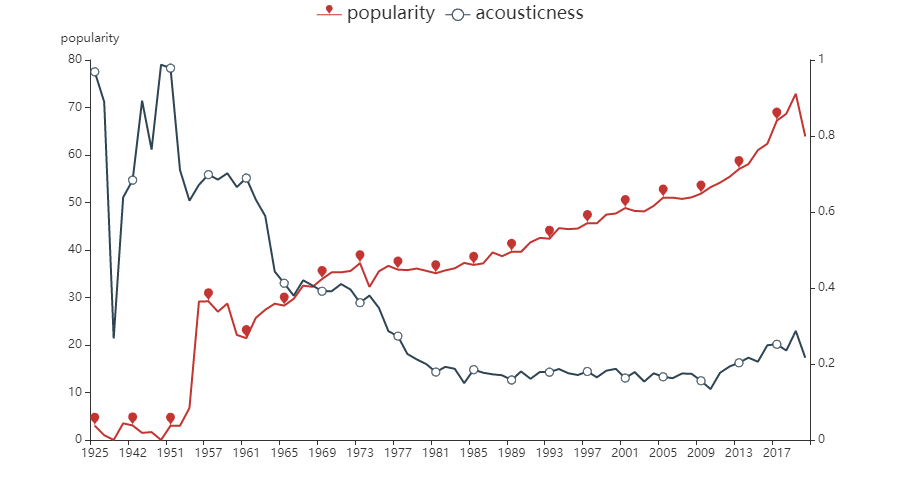
\includegraphics[width=0.42\linewidth]{pa}}
	\quad %默认情况下两个子图之间空的较少,使用这个命令加大宽度
	\subfigure[Circulation and duration]{
		\label{level.sub.2}
		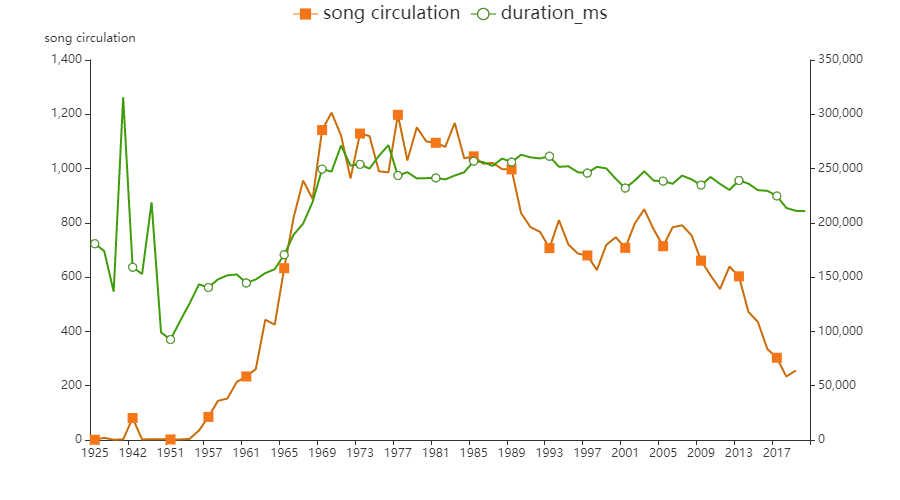
\includegraphics[width=0.42\linewidth]{sd}}
	%这里是空了一行,能够实现强制将四张图分成两行两列显示,而不是放不下图了再换行,使用\\也行。
	\subfigure[Loudness]{
		\label{level.sub.3}
		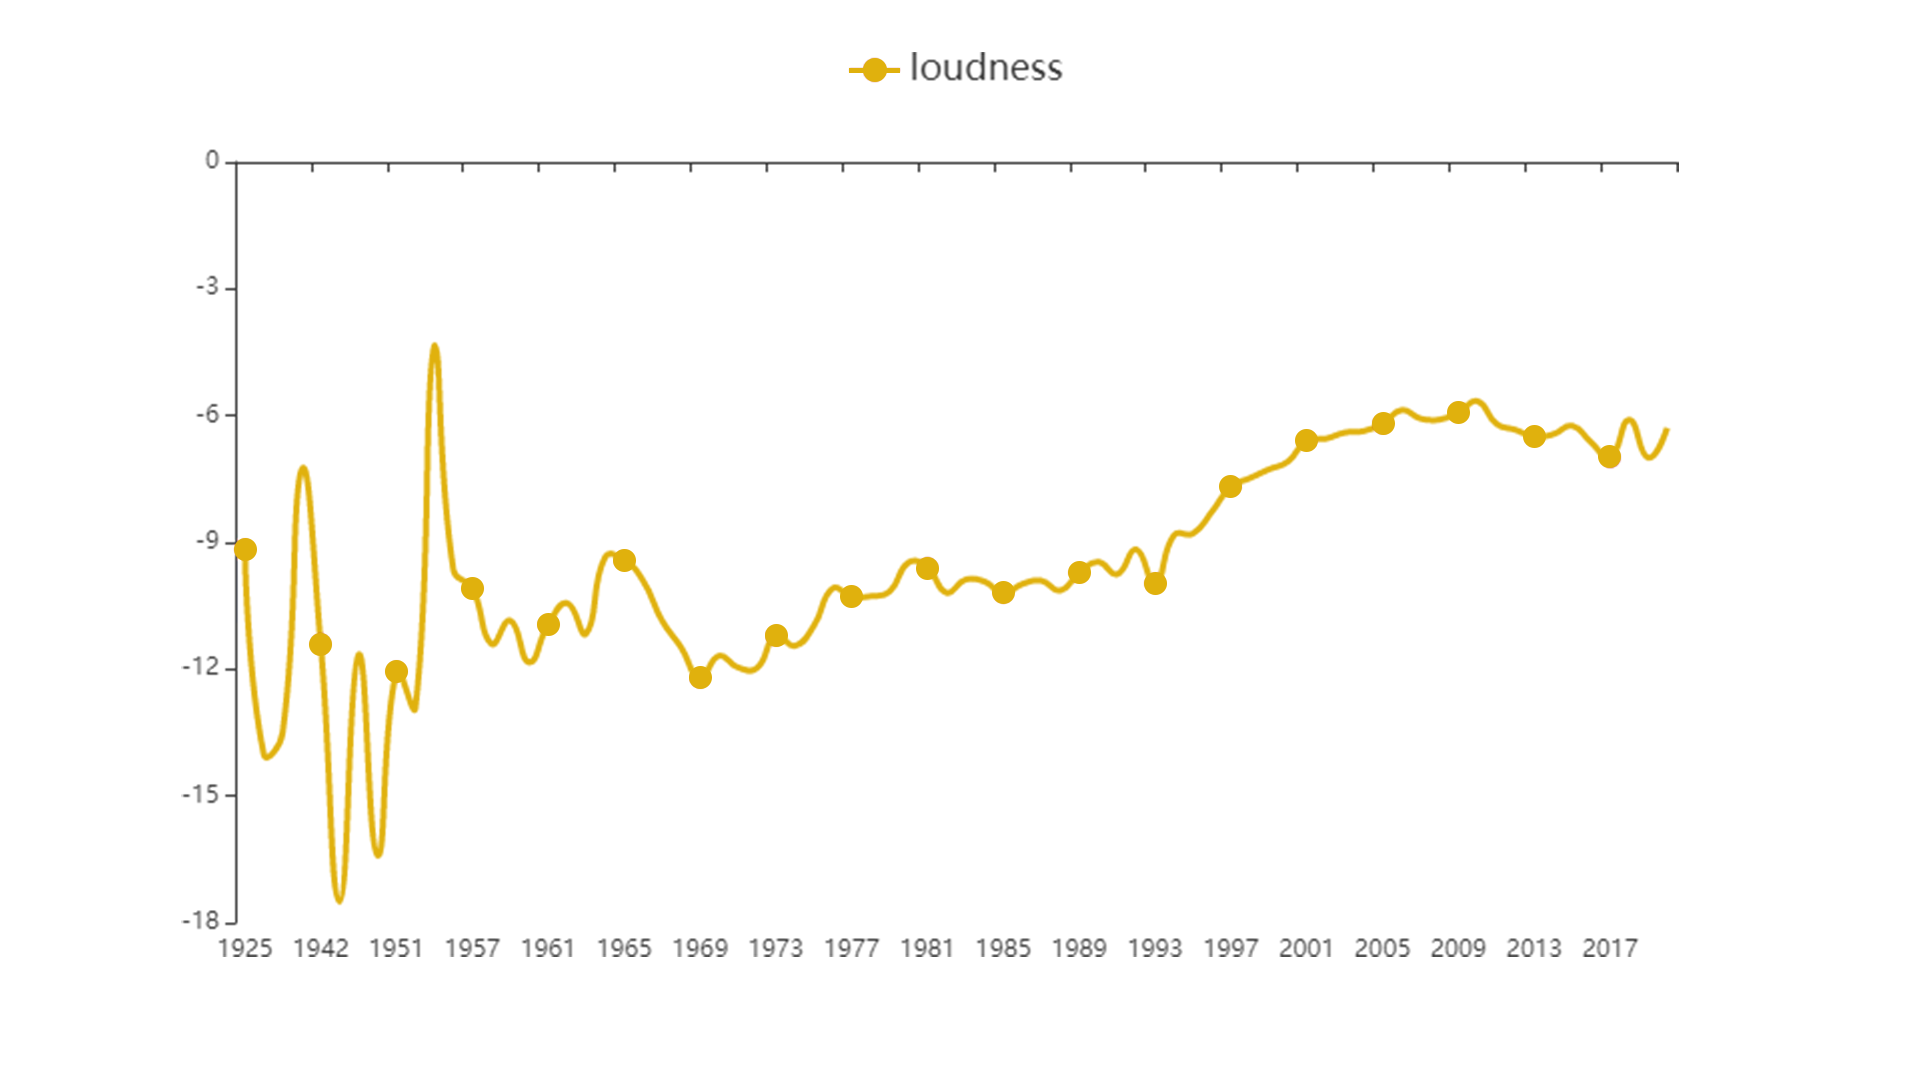
\includegraphics[width=0.42\linewidth]{l}}
	\quad
	\subfigure[The other characteristic]{
		\label{level.sub.4}
		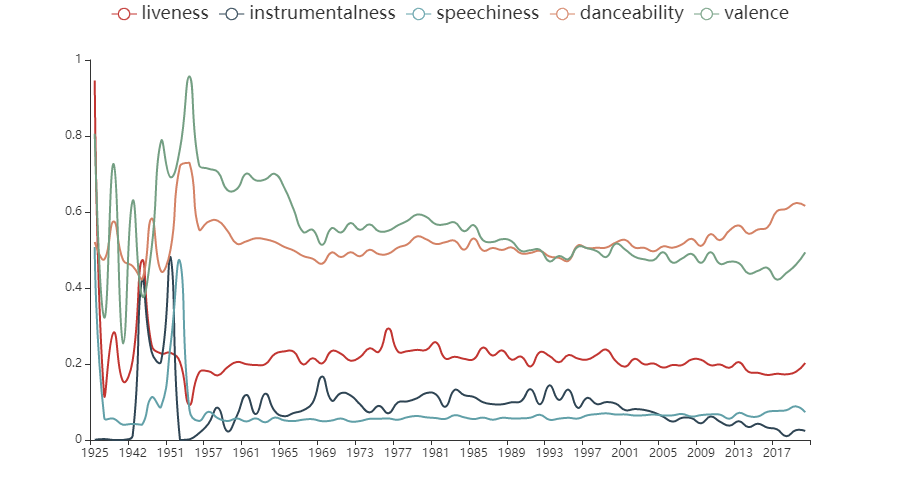
\includegraphics[width=0.42\linewidth]{most}}
	\caption{Characteristic time series diagram}
	\label{level}
\end{figure}
As can be seen from the figure, there was a sharp increase in acousticness, popularity and circulation in the 1940s, 1950s and 1960s respectively.Take the  indicator of acousticness as an example, on the basis of the dynamic influencers in Table 12, the saliva band was the dynamic influencer in the 1940s, which had a highe value of acoustic. So the acoustic of pop music in this period had a promoting effect from the band, which proved reliability of selecting dynamic influencer according to comprehensive dynamic evaluation index.
 
 
\section{External Factors}
In addition to being affected by artists, which is regarded as the internal influence of the music field, the external effect of social, political and technological changes can not be ignored.

\noindent%取消单段缩进
\textbf{Social Changes}

It can be seen from Figure 6 that Pop$/$Rock music developed rapidly in the 1950s and reached its peak from the 1960s to the 1970s, which is closely related to the social background at that time. After the end of the Second World War, the advent of peace made the population rise rapidly. The people born in this period are called baby boomers. Compared with their parents, the baby boomers are relatively rich in childhood and have more leisure time and more opportunities to develop their own subculture. Pop$/$Rock music is the product of this demand.

\noindent%取消单段缩进
\textbf{Political Changes}

There are also political reasons\upcite{4} for the above changes in Pop/Rock music. In the prosperous period of rock music, people tend to release their dissatisfaction with some policies and prejudices in rock music, which further promotes the popularity and development of Pop/Rock music.


\noindent%取消单段缩进
\textbf{Technological Changes}
 
The development of science and technology permeates all aspects of music. In summary, the influence of the development of science and technology on music is expressed in the following two aspects.
\begin{itemize}
	\item Change the way of music production and existence.
	\item Change the way of music spread and appreciation.
\end{itemize}
Take electronic music[5] as an example, from Figure 5 we can clearly see that its popularity has a leap in the 1960s. This is because the development and popularization of synthesizer technology has greatly reduced the cost and difficulty of music synthesis. And in the 1990s, the distribution of electronic music increased by leaps and bounds. In connection with the development of science and technology during that period, it can be known that the emergence of digital recording and media led to a sharp increase in distribution.
\begin{figure}[H]%图片
	\small
	\centering
	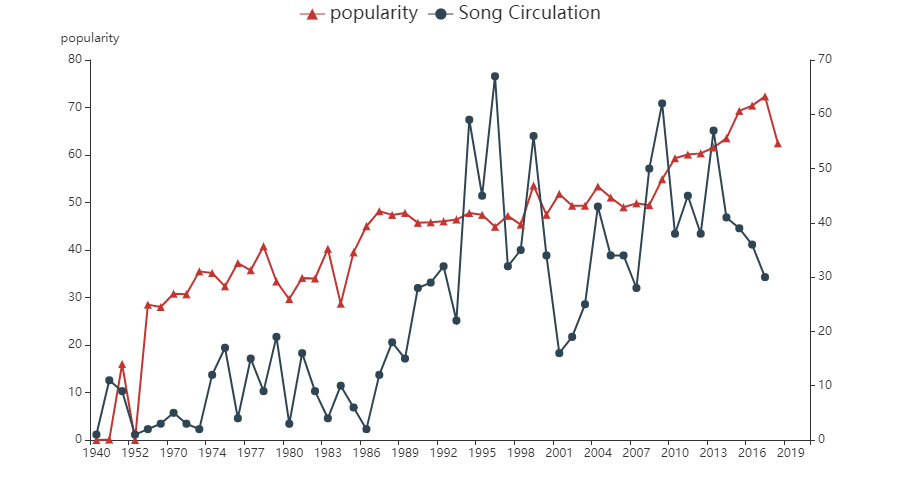
\includegraphics[height=5.2cm,width=14cm]{Ele}%图片名
	\caption{The popularity and circulation of electronic}\label{fig:7}%题注
\end{figure}
\section{Sensitivity Analysis}
In Section 6, we only consider the influencers and their corresponding followers to calculate the change of similarity by using characteristics. Now we study the effect of the fluctuation of the characteristic data on similarity.

 For the average growth rate of similarity, add Gaussian noise to the u1-u6 common factors obtained by factor analysis;
As for specific music characteristic similarity improvement rate, Gaussian noise is added to specific characteristic data.

Gaussian noise with mean value of 0 and variance variation is selected for 8 independent experiments, and the results are as follows.
\begin{figure}[H]%图片
	\small
	\centering
	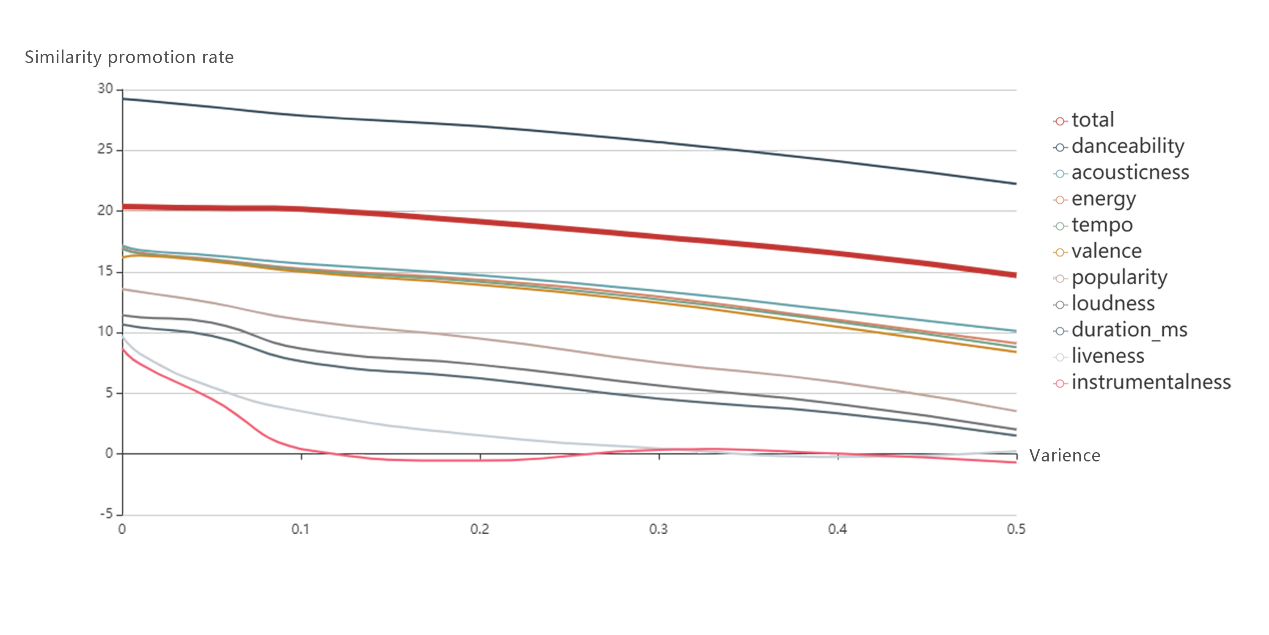
\includegraphics[width=14cm]{sen}%图片名
	\caption{Similarity promotion rate}\label{fig:7}%题注
\end{figure}
It can be seen that for the improvement of the average similarity, the injection of noise has little effect on its value, indicating that our model has good stability.

At the same time, for the results in Section 6, the characteristics with higher similarity, such as dance ability, can still maintain a higher promotion rate in the face of increased noise. While for the characteristic with lower similarity, such as instrumentalness, the obvious degree of the characteristic is gradually submerged in the big noise. And the promotion rate can also be ignored. This further shows that our model has strong robustness.

\section{Strength and Weakness}
\subsection{Strength}
\begin{itemize}
	\item The factor analysis method is used to reduce the dimensionality of the music characteristic. While maintaining 90$\%$ of the information in the data, the complexity of subsequent similarity calculation is greatly reduced, and the influence of the internal correlation of each characteristic on the result is also eliminated.
	\item We use weighted modified cosine similarity for similarity calculation, which not only considers the directional relationship of the multi-dimensional vector space, but also takes into account the size of the difference.
	\item Innovating on the basis of the original modified cosine similarity, we add the weight of each public factor to it, reducing the loss of data information.
	\item When analyzing the influencer's dynamic influence network, comprehensively consider intra-class and inter-class influence factors, and measure them from three aspects: time dimension, space depth, and influence breadth to make the influence evaluation standard more reasonable.
\end{itemize}
\subsection{Weakness}
\begin{itemize}
	\item In order to simplify the model, the influence of musicians' personal factors on music creation is not considered, such as their growth environment, education level, personality and so on. 
	\item Since the calculation of similarity requires multiple squaring and square root processing, the original noise of the data is amplified, which makes the final calculated value have a certain deviation;
\end{itemize}

\begin{thebibliography}{99}%参考文献
	\bibitem{1} Honglin Chu, Qicheng Liu, Chunxiao Mou. Improved Collaborative Filtering Recommendation Algorithm for Modified Cosine Similarity[J]. Journal of yantai university (natural science and engineering (2020)
	\bibitem{2}ishun Wang, Chunbin Wang, Minlun Yan. Comprehensive evaluation model on occupational situation of cities and towns units in various region based on the factor analysis method[J]. Mathematics in Practice and Theory 43(19), 10-18(2013)
	\bibitem{3}Fanjul-Hevia Arís;González-Manteiga Wenceslao;Pardo-Fernández Juan Carlos A non-parametric test for comparing conditional ROC curves[J]  SJES016794730698,2021
	\bibitem{4}Nancy Sue Love. Music and Democracy[M]. State University of New York Press, Albany, 1-16(2006)
	\bibitem{5}Nick Collins, Margaret Schedel, Scott Wilson. Electronic Music (Cambridge Introductions to Music)[M]. Cambridge University Press(2013)
\end{thebibliography}







\begin{appendices}
\section{Document to the ICM Society}
\rule{\textwidth}{02pt}

\noindent%取消单段缩进
To: ICM Society

\noindent%取消单段缩进
From: Team $\# 2104419$

\noindent%取消单段缩进
Date: February 8,2021

\noindent%取消单段缩进
Subject: The Influence of Music

\noindent%取消单段缩进
\rule{\textwidth}{02pt}
Dear Sir or Madam,

It is our great honor to be identified as the think tank to provide the analysis about the influence of music through networks. Based on the given data in the files, we develop some mathematic models to quantify the influence. Here are our analysis and conclusion.

First, we export the influence network diagram to understand the influence of music. The value of this method is as follows.
\begin{itemize}
	\item Clearly and intuitively show the relationship between influencers and followers.
	\item According to the thickness and shape of the arrow, it is easy to qualitatively analyze the influence depth and speed.
	\item On the basis of the color of the line, we can analyze the interaction between genres.
	\item It's visually to judge the estimated number of artists in the genre by observing the size of the circle.
\end{itemize}

Then we analyze the characteristics of the artist through modeling and solve the following problems.
\begin{itemize}
	\item How to measure the degree of similarity between artists and whether this degree of similarity is related to the genre.
	\item How to find indicators to distinguish different genres.
	\item How to identify revolutionaries and dynamic influencers.
	\item How to describe the change of each characteristic quantitatively.
\end{itemize}
As the amount of data increases, the difficulty of data processing will continue to increase, and the workload of various calculations and statistics will gradually increase. But at the same time, the statistical characteristics of the data will continue to increase, the phenomenon of data missing will get significantly improved, and the stability of the results obtained by the analysis is enhanced.
For the influence index of the dynamic influence network , we can first cluster the artists according to music genres and musical characteristics. And then we only need the influence relationship between each category. If the dimensionality of the music attribute is relatively high, we can still use factor analysis to reduce its dimensionality, but it will not be able to directly calculate the similarity level between the artists, so as to obtain the similarity between the classes of the music genres and the similarity within the classes. At this time, sampling calculation needs to be performed as the overall feature trend. For the next few questions, due to the increase in the amount of data, we basically do not need to perform data interpolation, and we cannot refine the change trend of each music characteristic over time. We need to use the common factor obtained in the second question as the final characteristics used for comparison. We also need to cluster music factions, and classify them into categories with higher feature similarity. And then just follow the previous method.

In the course of development of music, it is always affected by external political, economic, cultural and other factors. At the same time, it also demonstrates its influence in a subtle way. The production of music is closely related to culture. Music is rooted in culture, and it blends with, relies on and promotes each other. To sum up, we need to pay great attention to the influence of music.

We hope that the analysis and conclusions we provide can help you understand the impact of music more clearly. If you have any doubts about the above content, we will offer consultation at any time.

Sincerely, 
Team $\#$2104419
\end{appendices}
\end{document}
%% 
%% This work consists of these files mcmthesis.dtx,
%%                                   figures/ and
%%                                   code/,
%% and the derived files             mcmthesis.cls,
%%                                   mcmthesis-demo.tex,
%%                                   README,
%%                                   LICENSE,
%%                                   mcmthesis.pdf and
%%                                   mcmthesis-demo.pdf.
%%
%% End of file `mcmthesis-demo.tex'.
